\documentclass[border=5pt]{standalone}
\usepackage{amsmath,amssymb,mathtools}
\usepackage{tikz}
\usepackage{pgfplots}
\usepackage{pgf}
\begin{document}
	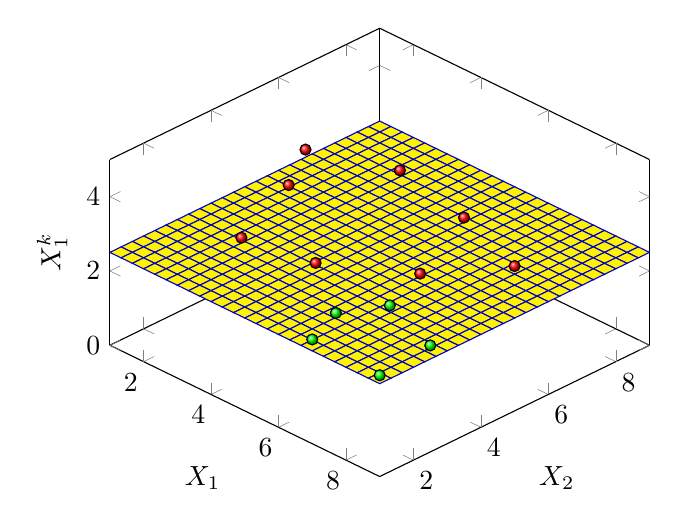
\begin{tikzpicture}
		\begin{axis}[
			view={45}{45}, % Adjust the viewing angle
			zmin=0, zmax=5,
			xmin=1,xmax=9,
			ymin=1,ymax=9,
			xlabel=$X_1$,
			ylabel=$X_2$,
			zlabel=$X_1^k$
			]
			\addplot3[only marks,ball color =red,
			mark = ball] coordinates {(8,3.2,4.05) (4.5,6.1,4) (9,5,3.9) (7,5.5,4.1) (6,2.1,3.94) (4.2,1.7,4) (3.5,3.8,4.18) (2.5,5.3,4.03)};
			\addplot3[only marks,ball color =green,
			mark = ball] coordinates {(5,3,1.04) (4.5,4.2,1) (5,5.3,0.94) (7,3,0.96) (7,4.5,1.1)};
			\addplot3[surf,domain=1:9, y domain=1:9,fill=yellow] {2.5};	
			\end{axis}
		\end{tikzpicture}
\end{document}